%====================================================
% ----                  Cap 3
%====================================================
\renewcommand{\caminhograficos}{aulas/cap_3/graficos}
\newcommand{\figCa}{
    \begin{figure}[H]
        \centering
        \includegraphics[width=0.8\textwidth]{fig-3.1.png}
        \caption{Gráfico de posição versus tempo para um MRU.}
        \label{fig:mru_veiculo}
    \end{figure}
}


\chapter{Movimento Retilíneo Uniforme (MRU)}
\label{cap:mru}
%----------------------------------------------------

O Movimento Retilíneo Uniforme (MRU) é o caso mais simples de movimento, servindo como base para a compreensão de dinâmicas mais complexas. Sua principal característica é a manutenção de uma velocidade constante ao longo de uma trajetória reta.

%=======================================
\section{Definição e Características}

No MRU, o móvel percorre distâncias iguais em intervalos de tempo iguais. Isso implica que:
\begin{itemize}
    \item A trajetória é uma linha reta.
    \item A velocidade escalar instantânea é constante e igual à velocidade escalar média ($v = v_m$).
    \item A aceleração é nula ($a = 0$), pois não há variação no módulo da velocidade.
\end{itemize}

%=======================================
\section{Função Horária da Posição}

A função horária permite determinar a posição ($s$) de um móvel em qualquer instante ($t$), desde que conheçamos sua posição inicial ($s_0$) e sua velocidade ($v$). Partindo da definição de velocidade média:

\begin{equation}
    v = \frac{\Delta s}{\Delta t} \implies v = \frac{s - s_0}{t - t_0}
\end{equation}

Considerando o instante inicial como $t_0 = 0$, temos:
\begin{equation}
    v = \frac{s - s_0}{t} \implies v \cdot t = s - s_0
\end{equation}

Isolando a posição final ($s$), obtemos a \textbf{Função Horária do MRU}\parencite{halliday2012}:

\begin{equation}
    s = s_0 + v \cdot t \label{eq:sorvete}
\end{equation}

\noindent Onde:
\begin{itemize}
    \item $s$: Posição final no instante $t$ (\unit{m}).
    \item $s_0$: Posição inicial no instante $t=0$ (\unit{m}).
    \item $v$: Velocidade escalar constante (\unit{m/s}).
    \item $t$: Tempo decorrido (\unit{s}).
\end{itemize}

\begin{example}
Um móvel parte da posição \unit{20}{m} com uma velocidade constante de \unit{5}{m/s}. Sua função horária será $s = 20 + 5t$. No instante $t = \unit{10}{s}$, sua posição será:
\begin{equation*}
    s = 20 + 5(10) = 20 + 50 = \unit{70}{m}
\end{equation*}
\end{example}

%=========================================================
\section{Análise de Dados e Tabelas}

A identificação de um Movimento Retilíneo Uniforme na prática ocorre através da coleta de posições em intervalos de tempo conhecidos. A principal característica matemática para identificar o MRU em uma tabela é observar que, para intervalos de tempo iguais ($\Delta t$), o deslocamento ($\Delta s$) também deve ser igual.

\subsection{Identificação Experimental}

Considere um móvel da \cref{fig:mru_veiculo}, cujas posições foram registradas conforme a tabela \cref{tab:dados_mru}. 

%==========================================
\figCa
%==========================================

\begin{table}[H]
    \centering
    \begin{tabular}{ccccccc}
        \toprule
        \textbf{Tempo} $t$ (s) & 0 & 1 & 2 & 3 & 4 & 5 \\ \midrule
        \textbf{Posição} $s$ (m) & 10 & 15 & 20 & 25 & 30 & 35 \\ \bottomrule
    \end{tabular}
    \caption{Registro de posições de um móvel em MRU.}
    \label{tab:dados_mru}
\end{table}

Ao analisarmos os dados da Tabela \ref{tab:dados_mru}, notamos que:
\begin{itemize}
    \item No instante $t=0$, a posição inicial é $s_0 = \unit{10}{m}$.
    \item A cada \unit{1}{s} que passa, a posição aumenta exatamente \unit{5}{m}.
    \item A razão $\frac{\Delta s}{\Delta t} = \frac{5}{1} = \unit{5}{m/s}$ é constante.
    \item Pode-se extrapolar os dados para qualquer instante $t$ usando a função horária $s = 10 + 5t$, de modo que, podemos prever a posição do móvel em instantes futuros ou passados, confirmando a natureza uniforme do movimento.
\end{itemize}

\subsection{Construção da Função Horária a partir de Dados}

Para montar a função horária $s = s_0 + v \cdot t$ a partir de uma tabela, seguimos dois passos simples:
\begin{enumerate}
    \item Identificamos $s_0$ observando o valor de $s$ quando $t=0$.
    \item Calculamos a velocidade $v$ escolhendo quaisquer dois pontos da tabela e aplicando $v = \frac{s_2 - s_1}{t_2 - t_1}$.
\end{enumerate}

No caso da tabela anterior:
\begin{equation*}
    s_0 = \unit{10}{m} \quad \text{e} \quad v = \frac{20 - 15}{2 - 1} = \unit{5}{m/s}
\end{equation*}
Logo, a função horária que descreve esses dados é: $s = 10 + 5t$.

%=========================================================
\section{Construção Gráfica do MRU}

A análise gráfica permite identificar visualmente o comportamento da velocidade e da posição. No MRU, como a função horária $s = s_0 + v \cdot t$ é uma equação do primeiro grau, sua representação no plano $s \times t$ será sempre uma reta inclinada.

\subsection{Gráficos de Posição por Tempo \texorpdfstring{($s \times t$)}{(s x t)}}

Para uma melhor compreensão, dividimos os gráficos de acordo com o sentido do movimento em relação à trajetória:

%=================================
\incluirgrafico{grafico_3.1.tex}
%=================================

Na \cref{fig:mru_prog}, a reta possui inclinação positiva, indicando que a posição do móvel aumenta com o tempo, caracterizando um movimento progressivo. Já na \cref{fig:mru_ret}, a reta tem inclinação negativa, mostrando que a posição diminui com o tempo, caracterizando um movimento retrógrado. 

\subsection{Gráfico Velocidade x Tempo \texorpdfstring{($v \times t$)}{(v x t)}}

No MRU, a velocidade é constante e diferente de zero. Graficamente, isso resulta em uma **reta horizontal**.

\textbf{Propriedade da Área:} A área entre a reta da velocidade e o eixo do tempo é numericamente igual ao deslocamento ($\Delta s$) do móvel no intervalo de tempo selecionado.

%=================================
\incluirgrafico{grafico_3.2.tex}
%=================================

%=========================================================
\section{Passo a Passo: Construindo o Gráfico no Caderno}

Para transformar a equação horária $s = 10 + 5t$ em um gráfico profissional usando régua e papel, siga estas etapas:

\subsection*{1º Passo: Construção da Tabela de Dados}
Não tente desenhar o gráfico direto. Primeiro, calcule pelo menos 3 pontos para garantir que sua reta não fique "torta".

\begin{table}[H]
    \centering
    \begin{tabular}{l|cccccc}
        \toprule
        \textbf{Instante $t$ (s)} & 0 & 1 & 2 & 3 & 4 & 5 \\ \midrule
        \textbf{Cálculo} & $10+5(0)$ & $10+5(1)$ & $10+5(2)$ & $10+5(3)$ & $10+5(4)$ & $10+5(5)$ \\
        \textbf{Posição $s$ (m)} & \textbf{10} & \textbf{15} & \textbf{20} & \textbf{25} & \textbf{30} & \textbf{35} \\ \bottomrule
    \end{tabular}
\end{table}

Com isso chegamos a \ref{tab:dados_mru} apresentada anteriormente, que é a base para a constrição gráfica. 

\subsection*{2º Passo: Definição da Escala (Uso da Régua)}
Este é o segredo para o gráfico caber na folha. Vamos converter os valores físicos em centímetros reais:

\begin{itemize}
    \item \textbf{No eixo horizontal (Tempo):} Adote \textbf{1 cm = 1 s}. Se seu gráfico vai até 10 s, desenhe uma linha de 10 cm.
    \item \textbf{No eixo vertical (Posição):} Adote \textbf{1 cm = 10 m}. Como precisamos chegar a 60 m, desenhe uma linha de 6 cm.
    \item \textbf{Observação:} Em situações diversas, é recomendado pegar o maior valor e subtrair do menor para encontrar o intervalo de variação, e então escolher pontos estratégicos dentro desse intervalo para garantir uma boa representação gráfica. Recomenda-se usar valores redondos para facilitar na hora de marcar os pontos. Por regra geral, é interessante escolher uma escala que permita que o gráfico ocupe a maior parte da folha, mas sem ultrapassá-la. Se os valores forem muito grandes ou muito pequenos, ajuste a escala para garantir que o gráfico seja legível e bem distribuído na página.
\end{itemize}

\subsection*{3º Passo: Plotagem e Destaques Geométricos}
Agora, transporte os dados para o papel seguindo estas orientações:

%=================================
\incluirgrafico{grafico_3.3.tex}
%=================================

\begin{enumerate}
    \item \textbf{Marque o $s_0$:} É o ponto onde a reta toca o eixo vertical (em $t=0$).
    \item \textbf{Trace as projeções:} Use linhas tracejadas para ligar o tempo à posição correspondente (ex: 6 s em 40 m).
    \item \textbf{Desenhe a reta:} Una os pontos. No MRU, a linha \textbf{deve} ser perfeitamente reta.
    \item \textbf{Observe que:} Os intervalos de tempo iguais (ex: 0-2 s, 2-4 s) correspondem a deslocamentos iguais (ex: 10 m). Isso é a essência do MRU.
    \item \textbf{Inclinação:} A inclinação da reta é diretamente proporcional à velocidade. Quanto mais inclinada, maior a velocidade. No exemplo, a inclinação é constante, confirmando o caráter uniforme do movimento. Com isso:
    \begin{equation}
        v = \tan(\alpha) = \frac{\Delta s}{\Delta t}  \implies v = \frac{40 - 20}{6 - 2} = 5m/s
    \end{equation}
\end{enumerate}

% --- FIM DA TEORIA ---
\newpage
%=========================================================
\section{Questões:}

Responda às questões abaixo com base nos conceitos de Movimento Retilíneo Uniforme (MRU) e na análise de seus gráficos.

\begin{enumerate}
    
    \item No gráfico de posição por tempo ($s \times t$) do MRU, a inclinação da reta em relação ao eixo horizontal fornece uma informação física fundamental. Essa inclinação é numericamente igual a:
    \begin{enumerate}[label=(\alph*)]
        \item A aceleração constante do móvel.
        \item A posição inicial ($s_0$) de onde o móvel partiu.
        \item A velocidade escalar média do movimento.
        \item O deslocamento total efetuado pelo corpo.
    \end{enumerate}

    \item Analise a função horária $s = 50 - 2t$ (unidades no SI). Sobre o movimento descrito por essa equação, é correto afirmar que:
    \begin{enumerate}[label=(\alph*)]
        \item O movimento é progressivo, pois a posição inicial é positiva.
        \item O móvel encontra-se em repouso no instante $t = 25$ s.
        \item O movimento é retrógrado, indicando que o móvel caminha contra a orientação da trajetória.
        \item A velocidade do móvel aumenta em 2 m/s a cada segundo que passa.
    \end{enumerate}

    \item Durante a construção de um gráfico $s \times t$, um aluno percebe que a reta cruza o eixo horizontal exatamente no valor $t = 4$ s. O significado físico desse ponto de intersecção é:
    \begin{enumerate}[label=(\alph*)]
        \item O instante em que o móvel inverte o sentido do seu movimento.
        \item O instante em que o móvel passa pela origem das posições ($s = 0$).
        \item O momento em que o cronômetro foi acionado pelo observador.
        \item O ponto de maior velocidade atingida pelo móvel na trajetória.
    \end{enumerate}

    \item Por que é indispensável manter uma escala constante (ex: cada 1 cm na régua valendo sempre 10 m no papel) ao desenhar os eixos de um gráfico de MRU?
    \begin{enumerate}[label=(\alph*)]
        \item Apenas por uma questão de estética e organização visual da apostila.
        \item Para garantir que a reta do gráfico sempre comece na origem (0,0).
        \item Para evitar que a representação visual da velocidade sofra distorções, mantendo a linearidade da reta.
        \item Para que o ângulo de inclinação seja obrigatoriamente de $45^\circ$.
    \end{enumerate}

    \item Se dobrarmos o valor da velocidade de um móvel em MRU, como essa alteração será observada visualmente no gráfico de posição por tempo?
    \begin{enumerate}[label=(\alph*)]
        \item A reta se tornará uma parábola voltada para cima.
        \item A reta ficará mais "em pé" (maior inclinação em relação ao eixo horizontal).
        \item A reta se deslocará verticalmente, alterando o valor de $s_0$.
        \item A reta se tornará perfeitamente horizontal, paralela ao eixo do tempo.
    \end{enumerate}

\end{enumerate}

%=========================================================
\section{Exercícios:}

\begin{enumerate}

    % Exercício 1: Interpretação de Tabela
    \item Um móvel realiza um movimento retilíneo cuja tabela de posições em função do tempo é dada abaixo:
    \begin{center}
        \begin{tabular}{l|ccccc}
            \toprule
            $t$ (s) & 0 & 2 & 4 & 6 & 8 \\ \midrule
            $s$ (m) & 20 & 30 & 40 & 50 & 60 \\ \bottomrule
        \end{tabular}
    \end{center}
    Determine a velocidade escalar do móvel e escreva sua função horária das posições.

    % Exercício 2: Função Horária Simples
    \item Um ponto material movimenta-se sobre uma trajetória retilínea obedecendo à função horária $s = -15 + 3t$ (SI). Determine:
    \begin{enumerate}[label=\alph*)]
        \item A posição inicial e a velocidade.
        \item A posição do móvel no instante $t = 10$ s.
        \item O instante em que o móvel passa pela origem das posições ($s = 0$).
    \end{enumerate}

    % Exercício 3: Distância e Tempo
    \item Um carro mantém uma velocidade constante de \qty{72}{km/h} em uma rodovia retilínea. Calcule a distância percorrida pelo veículo após \qty{15}{minutos} de viagem.

    % Exercício 4: Análise Gráfica (Progressivo/Retrógrado)
    \item Um objeto move-se de acordo com o gráfico $s \times t$ abaixo. Determine a velocidade do objeto e classifique o movimento como progressivo ou retrógrado.
    \cref{fig:exemplo_grafico_2026}
    % (Inserir aqui o código TikZ simplificado da reta descendo de 40 para 0 em 8s)

    \begin{figure}[H]
    \centering
    \begin{tikzpicture}
        \begin{axis}[
            axis lines = left,
            xlabel = {$t$ (s)},
            ylabel = {$s$ (m)},
            % Ajuste para 5 segundos
            xmin=0, xmax=6,
            ymin=0, ymax=50,
            xtick={0, 1, 2, 3, 4, 5},
            ytick={0, 10, 20, 30, 40},
            grid = major,
            grid style = {dashed, gray!30},
            width=0.8\textwidth, height=7cm
        ]

            \addplot [domain=0:5, thick, red] {40 - 8*x} 
                node[pos=0.8, sloped, above] {};

            \draw [dashed, black!60] (axis cs:3.33,0) -- (axis cs:3.33,13.33);
            \draw [dashed, black!60] (axis cs:0,13.33) -- (axis cs:3.33,13.33);
            
        \end{axis}
    \end{tikzpicture}
    \caption{Gráfico que descreve o movimento de um objeto móvel. \label{fig:exemplo_grafico_2026}}
\end{figure}

    % Exercício 5: Conversão de Unidades
    \item A função horária de um projétil é $s = 100 + 20t$ (SI). Qual será a posição deste projétil, em quilômetros, após \qty{2}{minutos} de movimento?

    % Exercício 6: Comparação de Velocidades
    \item Dois móveis, A e B, possuem as seguintes funções horárias: $s_A = 10 + 2t$ e $s_B = 40 - 3t$ (SI). Determine o instante e a posição em que esses dois móveis se encontram.

    % Exercício 7: Velocidade Média em Trechos
    \item Um ciclista percorre \qty{4}{km} com velocidade constante de \qty{12}{km/h} e, em seguida, mais \qty{6}{km} com velocidade constante de \qty{18}{km/h}. Determine o tempo total do percurso.

    % Exercício 8: Gráfico de Velocidade
    \item Desenhe o gráfico de velocidade por tempo ($v \times t$) para um móvel que se desloca segundo a função $s = 50 - 5t$ (SI), para o intervalo de 0 a \qty{10}{s}.

    % Exercício 9: Ultrapassagem
    \item Um trem de \qty{100}{m} de comprimento atravessa uma ponte de \qty{50}{m} com velocidade constante de \qty{15}{m/s}. Quanto tempo o trem leva para atravessar completamente a ponte?

    % Exercício 10: Desafio de Escala
    \item Um aluno deseja construir um gráfico para a função $s = 5 + 25t$. Se ele utilizar uma régua e adotar a escala de \qty{1}{cm} para cada \qty{5}{m} no eixo vertical, a que altura (em cm) estará o ponto correspondente ao instante $t = 3$ s?

\end{enumerate}

%=========================================================
\section{Problemas:}

\begin{enumerate}

    % Problema 1: Encontro de Móveis com Sentidos Opostos
    \item Duas cidades, A e B, estão separadas por uma distância de \qty{300}{km}. No mesmo instante, um carro parte da cidade A em direção a B com velocidade constante de \qty{80}{km/h}, enquanto um caminhão parte de B em direção a A com velocidade constante de \qty{70}{km/h}. 
    \begin{enumerate}[label=\alph*)]
        \item Determine as funções horárias das posições para ambos os veículos, adotando a cidade A como a origem ($s=0$).
        \item Calcule após quanto tempo os veículos se encontrarão na rodovia.
        \item Qual a posição do ponto de encontro em relação à cidade A?
    \end{enumerate}

    % Problema 2: Ultrapassagem e Comprimento
    \item Um trem de carga de \qty{200}{m} de comprimento viaja com velocidade constante de \qty{36}{km/h}. Ele deve atravessar completamente um túnel de \qty{100}{m} de extensão. 
    \begin{enumerate}[label=\alph*)]
        \item Converta a velocidade do trem para metros por segundo (\unit{m/s}).
        \item Qual é a distância total que o trem deve percorrer para que o último vagão saia completamente do túnel?
        \item Quanto tempo, em segundos, dura a travessia completa?
    \end{enumerate}

    % Problema 3: Interpretação de Gráficos de Encontro
    \item Dois móveis, $M_1$ e $M_2$, caminham sobre a mesma trajetória retilínea. O gráfico abaixo representa as suas posições em função do tempo:
    \cref{fig:referencia_grafico_desafio}
    
    \begin{center}
    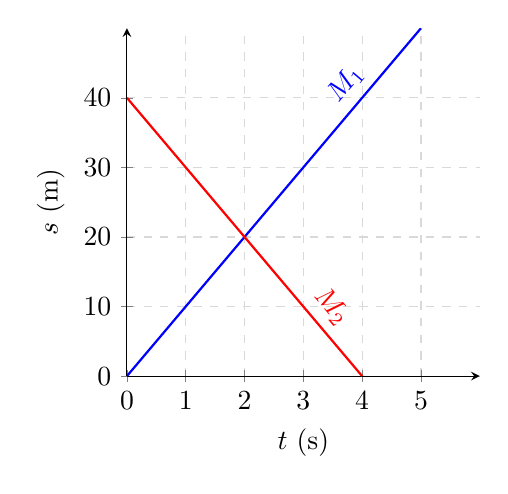
\begin{tikzpicture}
        \begin{axis}[
            axis lines = left,
            xlabel = {$t$ (s)},
            ylabel = {$s$ (m)},
            xmin=0, xmax=6,
            ymin=0, ymax=50,
            xtick={0,1,2,3,4,5},
            ytick={0,10,20,30,40},
            grid = major,
            grid style={dashed, gray!30},
            width=0.5\textwidth, height=6cm
        ]
            % Móvel 1 (Parte do 0 com v=10)
            \addplot [domain=0:5, thick, blue] {10*x} node[pos=0.8, sloped, above] {$M_1$};
            % Móvel 2 (Parte do 40 com v=-10)
            \addplot [domain=0:4, thick, red] {40 - 10*x} node[pos=0.8, sloped, above] {$M_2$};
        \end{axis}
    \end{tikzpicture}
    \label{fig:referencia_grafico_desafio}
    \end{center}
    
    A partir da análise do gráfico, determine:
    \begin{enumerate}[label=\alph*)]
        \item As funções horárias de $M_1$ e $M_2$.
        \item O instante exato em que os móveis se cruzam.
        \item A classificação (progressivo ou retrógrado) de cada movimento.
    \end{enumerate}

\end{enumerate}